\section{Theorie}
\label{sec:Theorie}

% In knapper Form sind die physikalischen Grundlagen des Versuches, des Messverfahrens, sowie sämtliche für die Auswertung erforderlichen Gleichungen darzustellen. (Keine Herleitung)

% (eventuell die Aufgaben)

% Der Versuchsaufbau: Beschreibung des Versuchs und der Funktionsweise (mit Skizze/Bild/Foto)
\subsection{Dampfdruckkurve und Verdampfungswärme}
\label{ssec:a}
Es gibt insgesamt drei Aggregatzustände, flüssig, fest und gasförmig.
Diese werden als sogenannte Phasen angesesehen, da sie in einem räumlich abgegrenzten Bereich einen physikalisch homogenen Zustand einnehmen.
Diese Phasen sind deutlich in einem Zustandsdiagramm erkennbar.
Darin wird die Temperatur $T$ gegen den Druck $p$ aufgetragen.
In \autoref{fig:skizze_1} ist ein solches Diagramm dargestellt.

\begin{figure}
    \centering
    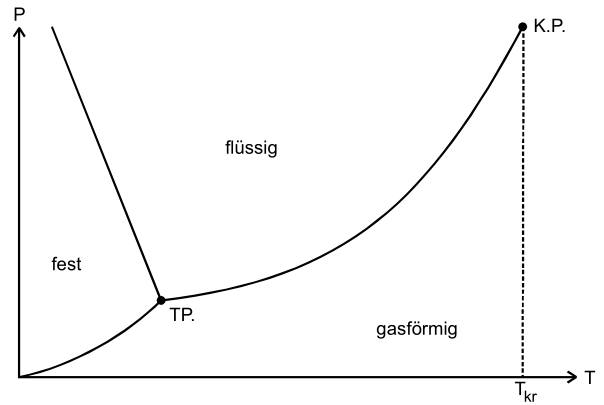
\includegraphics[width=\textwidth/2]{images/bild1.png}
    \caption{Quantitative Darstellung eines Zustanddiagramms von Wasser \cite{V203}}
    \label{fig:skizze_1}
\end{figure}

Innerhalb der Bereiche, die durch die Kurven abgegrenzt werden, sind $T$ und $p$ frei wählbar.
In diesem Experiment ist der Phasenübergang von flüssig zu gasförmig, sowie umgekehrt, im Fokus.
Die Kurve, die durch den Tripelpunkt TP und den Kurvenpunkt begrenzt ist, wird Dampfdruckkurve genannt und wird in diesem Experiment genauer untersucht.
Auf der Dampfdruckkurve befinden sich beide Zustände in einem Gleichgewicht, sie koexistieren.
Der wesentliche Parameter dieser Kurve wird Verdampfungswärme $L$ genannt, dieser soll im Verlauf der Auswertung bestimmt werden.
Auf die ganze Dampfdruckkurve bezogen ist $L$ nicht konstant, aber in dem Bereich, der hier betrachtet wird, kann $L$ als konstant angenommen werden.
Im Folgenden wird erklärt, wie die Dampfdruckkurve zustande kommt.

Sollte eine Flüssigkeit in einem evakuiertes Gefäß beginnen zu verdampfen, erhöht sich gleichzeitig auch der Druck. Das Volumen bleibt konstant, aber der Gasanteil steigt, also muss der Druck ansteigen.
Damit die Moleküle die Flüssigkeit verlassen können, benötigen sie eine hohe Energie, diese muss zugefügt werden.
Die Verdampfungswärme $L$ ist ein Maß für die benötigte Energie.
Sie ist definiert als die Energie, die benötigt wird, ein Mol Flüssigkeit in die gasförmige Phase umzuwandeln.
Wenn die Bedingungen, unter denen das Experiment stattfindet, konstant bleiben, stellt sich ein Druck ein, der sich nicht mehr ändert.
Dieser Druck wird Sättigungsdampfdruck genannt und beschreibt den Druck, bei denen flüssige und gasförmige Phase unveränderlich nebeneinander existieren.
Wird die Temperatur erhöht, verlassen noch mehr Moleküle die Flüssigkeit und der Sättigungsdampfdruck steigt ebenfalls an.
Für diese gesättigten Gase gilt die allgemeine Gasgleichung allerdings nicht mehr.

\begin{equation}
    pV = RT
    \label{eq:gas:gl}
\end{equation}

\subsection{Die Clausius-Clapeyronsche Gleichung}
\label{ssec:b}

Um eine Gasgleichung für dieses System zu gewinnen muss der ganze Kreisprozess, wie in \autoref{fig:skizze_2} durchgerechnet werden.

\begin{figure}
    \centering
    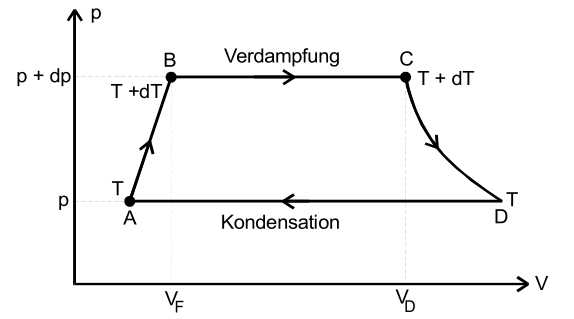
\includegraphics[width=\textwidth/2]{images/bild2.png}
    \caption{Darstellung einer Verdampfung und Kondensation eines Stoffes \cite{V203}}
    \label{fig:skizze_2}
\end{figure}

Der Prozess beginnt im Punkt A.
Dort wird eine Wärmemenge $dQ_\text{AB}$ zugefügt, sodass Temperatur, Druck und Volumen ansteigen.
Danach wird die Verdampfungswärme $L$ verwendet, um die Flüssigkeit, unter isobaren und isothermen Umständen, zu verdampfen.
Schließlich wird eine Wärmemenge $dQ_\text{CD}$ entfernt, der Stoff besitzt wieder die ursprüngliche Temperatur, der Druck sinkt und das Volumen steigt.
Damit der Stoff sein ursprüngliches Volumen einnimmt, kondensiert er unter Zuführung von Mechanischer Energie.
Wird die gesamte zugeführt Wärmemenge summiert, ergibt sich

\begin{equation}
    \dif{Q_\text{ges}} = C_\text{F} \dif{T} - C_\text{D} \dif{T} + \dif{L}.
    \label{eq:waerme}
\end{equation}

Dabei ist $C_\text{F}$ die Molwärme der Flüssigkeit und $C_\text{D}$ die Molwärme des Dampfes.
Die Wärmewenge wird nun mit der geleisteten Arbeit

\begin{equation}
    A = \dif{p} \left(V_\text{D} - V_\text{F}\right)
    \label{eq:arbeit}
\end{equation}

gleichgesetzt und nach einer längeren Herleitung ergibt sich

\begin{equation}
    \dif{p} \left(V_\text{D} - V_\text{F}\right) = \frac{L}{T} \dif{T}.
    \label{eq:clausius}
\end{equation}

Diese Differenzialgleichung wird Clausius-Clapeyronsche Gleichung genannt und beschreibt die die Druckkurve dieses Prozesses.
Es ist ziemlich umständlich diese Gleichung zu lösen, daher wird sie in den nächsten Schritten vereinfacht.
Unter gewissen Umständen, wie die während dieses Experiments, kann die Gleichung auf eine einfachere Form gebracht werden.
Nach einigen Annahmen, die nicht näher beschrieben werden, kann die Clausius-Clapeyronsche Gleichung auf

\begin{equation}
    \ln p = \frac{-L}{R} \frac{1}{T} + \text{const}
    \label{eq:clausius2}
\end{equation}

vereinfacht werden, bzw in die Form

\begin{equation}
    p =  p_0 \exp{\frac{-L}{R} \frac{1}{T}}
    \label{eq:clausius3}
\end{equation}

gebracht werden.